\documentclass{IEEEcsmag}

\usepackage[colorlinks,urlcolor=blue,linkcolor=blue,citecolor=blue]{hyperref}

\usepackage{upmath}
\usepackage{amsmath}
\usepackage{url}
\usepackage{breakurl}
\usepackage[inkscapeformat=png]{svg}
% \usepackage[breaklinks]{hyperref}
% \def\UrlBreaks{\do\/\do-}

\jvol{Vol. 2}
\jnum{CS 611}
\paper{8}
\jmonth{April}
\jname{THREADS}
\pubyear{2023}
\newtheorem{theorem}{Theorem}
\newtheorem{lemma}{Lemma}

\setcounter{secnumdepth}{0}

\begin{document}
\setcounter{page}{1}
\title{The Shape of Learning}

\author{Tyler Trogden}
\affil{Brigham Young University}

\markboth{The Shape of Information}{}

\begin{abstract}
\end{abstract}

\maketitle

\chapterinitial{}


\section{Introduction}
  One may reasonably ask, what sort of information can we obtain by studying the
  shape of a given data set? The answer is that, it depends! The shape of a data set
  could give us valuable information, if we ``look'' at it in the right way. But admittedly
  there are myriad ways to ``look'' at a data set, from simple statistical measures
  to more complex machine learning algorithms. But perhaps the most intuitive way
  to ``look'' at a data set is to ``visualize" it. This is where the shape can be
  most easily exploited.
  
  Take as a simple example the set of points in the plane that are equidistant from 
  the origin, i.e., 
  
  \[
    S = \Big\{ (\cos^2 \theta, \sin^2 \theta) \,\big|\, \theta \in [-\pi, \pi) \Big\}.
  \]

  Plotting these points we would find that they form a circle. This is not surprising
  as we know that the distance from the origin to any point on the circle is the same.
  But what if we had no idea how these points were generated? What if we didn't know
  that they could be described by the trigonometric relationship above? After plotting
  them, we would still be able to see that they form a circle. Knowing this, we could
  then use this information to make predictions about the data set, or even to generate
  new points in the set. Essentially we have learned something about the process that
  generated the data that we did not previously know.

  Granted, the above example is a bit contrived. But it does illustrate the point that
  the shape of a data set can be used to learn something about the process that generated
  the data. However, we require techniques that can be applied to more complex data sets,
  data sets that, as a whole, are not necessarily as easy to visualize as the above example.
  How would you do this then for a data set that contains more than two dimensions? Or three 
  dimensions? One hundred? One million? Or even for data that is not a subset of the reals,
  but a more complex object such as a graph? 

  This is where topological data analysis (TDA) comes in. TDA is a mathematical framework that
  analyzes the shape and structure of data using tools from topology, a branch of mathematics
  that studies the properties of spaces that are preserved under continuous transformations.
  TDA has a wide range of applications in fields such as biology, neuroscience, computer science,
  and physics, among others.

  TDA can tell us many things about the data, depending on the specific techniques used and the context in 
  which they are applied. Here are a few examples:

  \begin{enumerate}
      \item TDA can help us identify the presence of patterns or structures in the data that are not readily 
      apparent from simple visual inspection or standard statistical methods.
      \item TDA can reveal the relationships between different parts of the data, including clusters, 
      subgroups, and outliers.
      \item TDA can provide a summary or abstraction of the data that captures the essential features of the 
      underlying structure, making it easier to interpret and communicate the results.
      \item TDA can help us understand how the data changes over time or under different conditions, 
      revealing the dynamics and evolution of the underlying process.
  \end{enumerate}

Overall, TDA is a powerful tool for extracting meaningful insights from complex and high-dimensional data, 
and it is increasingly being used in many different fields to uncover hidden structures and relationships 
that would otherwise be difficult to detect. For these reasons, it is no surprise that researchers are 
beginning to explore the use of TDA in the field of machine learning. In this article, we will discuss the
history of TDA, beginning from its origins in topology, and some of its applications in machine learning today.
Particularly, we will give special attention to the ideas of how the main tools of TDA, namely persistence homology,
were formed and how they might be used to probe the structural and functional properties of neural networks, in hopes 
of gaining insight into how they learn, i.e., finally giving a possible answer to that most difficult of questions,
``Why is a neural network doing what it's doing?".

\section{The Birth of Topology}
  \subsection{Leonhard Euler}
    Leonhard Euler (1707-1783) \cite{boyer2023euler} was a Swiss mathematician, physicist, and engineer who 
    made important contributions to many areas of mathematics, including calculus, number theory, graph 
    theory, and geometry, and who is considered as the founder of the mathematical field of topology.

    Among Euler's many achievements are the development of the notation for mathematical functions, the 
    discovery of the constant $e$, the formulation of Euler's formula (which relates exponential functions, 
    trigonometric functions, and complex numbers), and the solution of the famous Basel problem. He also made 
    important contributions to the study of mechanics, optics, and astronomy.

    Euler was born in Basel, Switzerland to Paul Euler and his wife Margaret Brucker. The oldest of 
    four children, Euler was expected to one day take up his father's occupation as that of a pastor in 
    the Protestant church. This perhaps was one of the key aspects of Euler's life that would allow him the
    opportunity of pursuing a university education, since being a pastor would require theological training.
    For this same reason Euler's own father, Paul, had received a university education from the University of 
    Basel some years earlier, where he had the opportunity to take courses in mathematics from none other than 
    Jacob Bernoulli \cite{oconn1998euler}.
    
    Given these facts it seems safe to assume that Paul also had an interest in mathematics and was well enough 
    trained that he began young Euler's primary education in the subject. However, it wasn't until some time 
    later that Euler would begin a more rigorous study of mathematics at the University of Basel himself, at 
    the ripe age of fourteen.

    Being enrolled in the university, Euler was expected eventually to study theology after obtaining a more
    general education, in which time he had the chance to take fundamental courses in mathematics from 
    Johann Bernoulli, the younger brother of the then deceased Jacob Bernoulli. It seems clear that Johann
    could see a talent in young Euler for mathematics, and upon graduating and beginning more advanced studies,
    Euler and Johann were able to convince Paul, that Euler should devote his studies and ultimately his career
    to mathematics.
  
    \subsubsection{The Bridges of Königsberg}
      The Bridges of Königsberg problem is a famous puzzle in mathematics that concerns the layout of seven 
      bridges in the city of Königsberg (now known as Kaliningrad, Russia). The problem was first posed in the 
      early 18th century by Euler.
    
      At the time, Königsberg was a city located on both sides of the Pregel River, which was crossed by seven 
      bridges (as seen in \ref{fig:seven_bridges}). The problem was to find a walk through the city that 
      would cross each bridge exactly once and return to the starting point.

      \begin{figure}
          \centering
          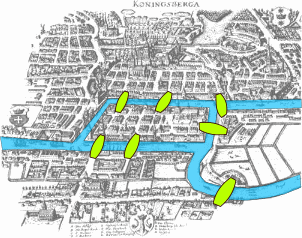
\includegraphics[width=0.35\textwidth]{konig_bridges.png}
          \caption{Seven bridges at the time of Euler. Attribution:
                    Bogdan Giuşcă,
                    \href{http://creativecommons.org/licenses/by-sa/3.0/}{CC BY-SA 3.0}}
          \label{fig:seven_bridges}
      \end{figure}
    
      Euler approached the problem using a new mathematical technique called graph theory, which he had 
      recently invented. He represented the city as a graph, with the land areas as vertices and the bridges 
      as edges connecting them. He then used this graph to investigate the properties of the underlying topological space.
    
      Euler observed that for a walk to cross each bridge exactly once, each vertex of the graph must be 
      visited an even number of times, except for the starting and ending vertices, which must be visited an 
      odd number of times. However, in the case of Königsberg, each of the four land areas connected by the 
      bridges had an odd number of bridges leading to it, which meant that it was impossible to find such a 
      walk.
    
      This was a significant discovery, as it marked the first time that graph theory had been used to solve a 
      problem in mathematics. It also gave birth to the idea that the only relevant features of the problem
      weren't distances or angles, as in geometry, but relative position and connectivity. As long as the 
      problem could be posed as a graph, it did not matter how the graph was deformed as long as the edges and
      vertices were not changed, which gives rise to the very fundamental concept of homeomorphism in topology,
      i.e., a bi-continuous bijection between topological spaces.

      But even though Euler had solved (in the negative) the Bridges of Königsberg problem in the firs half of 
      the 18th century, and introduced some very basic notions of topology, it wouldn't be until over a century 
      later till other significant contributions to the field would be made.

\section{The Abstraction of Topology}
  At this point, the fields of general topology and algebraic topology were not separate fields of study.
  It seems that algebraic topology was hardly conceived of at all as a separate field. However, small steps 
  were being made towards its development, with the increasing interest in questions regarding the surfaces of
  combinatorial arrangements of polyhedra in space \cite{carlson2007histTop}. One such scientist whose interest
  was piqued by these questions was the German mathematician, Bernhard Riemann, whose work would later go on
  to inspire the work of Enrico Betti, and in turn, Henri Poincaré.

  \subsection{Bernhard Riemann}
    Bernhard Riemann was a German mathematician born on September 17, 1826, in Breselenz, a village near Dannenberg in 
    the Kingdom of Hanover. He is best known for his pioneering work in the field of mathematics, particularly his 
    contributions to number theory, geometry, and mathematical analysis.

    Riemann grew up in a poor family, and his early education was mainly received from his father, who was a Lutheran 
    minister. He showed great talent in mathematics at an early age and was sent to the Gymnasium in Hanover for his 
    secondary education.

    In 1846, Riemann began studying at the University of Göttingen, where he was mentored by the mathematicians Carl 
    Friedrich Gauss and Christian Gerling. In 1851, he received his Ph.D. from the University of Göttingen with a 
    thesis on the theory of complex functions. His thesis introduced what is now known as the Riemann surface, a 
    geometric object that provides a way of extending complex functions to higher dimensions.

    In 1854, Riemann published a groundbreaking paper on the distribution of prime numbers, which is now considered a 
    fundamental contribution to number theory. The paper introduced the Riemann zeta function, which is a mathematical 
    function that provides information about the distribution of prime numbers. The Riemann hypothesis, which remains 
    unsolved to this day, is one of the most famous unsolved problems in mathematics and is related to the zeros of 
    the Riemann zeta function.

    Riemann also made important contributions to differential geometry and mathematical physics. In 1859, he 
    introduced the concept of Riemannian geometry, which is a mathematical framework for studying the curvature of 
    spaces. This work had a significant impact on the development of the theory of relativity.

    Riemann suffered from health problems throughout his life, including a severe lung condition. He died on July 20, 
    1866, in Selasca, Italy, at the age of 39. Despite his short life, Riemann's work had a profound impact on 
    mathematics and physics and remains an active area of research to this day.
  
  \subsection{Enrico Betti}
    Enrico Betti (1823-1892) \cite{editors2002betti} was an Italian mathematician, best known for his work in topology 
    and algebraic geometry. He was born in Pistoia, Italy and received his education in mathematics at the University 
    of Pisa.

    Betti's most significant contribution to mathematics is his work on the topology of surfaces. In 1866, he 
    introduced what is now known as the Betti numbers, which are a set of numerical invariants that can be used 
    to describe the topology of a space. These numbers are now fundamental in the study of algebraic topology.

    In addition to his work in topology, Betti also made important contributions to algebraic geometry and the 
    theory of elasticity. He was awarded the Royal Society's Copley Medal in 1890 for his contributions to 
    mathematics.

    Betti's legacy continues to influence modern mathematics, particularly in the areas of topology and 
    algebraic geometry.

    \subsubsection{Betti Numbers}

  \subsection{Henri Poincaré}
    Henri Poincaré (1854-1912) was a French mathematician, physicist, and philosopher of science. He made 
    important contributions to many areas of mathematics, including topology, algebraic geometry, and the theory 
    of differential equations. He is also known for his work in mathematical physics, including his formulation 
    of the principle of relativity and his discovery of chaotic behavior in dynamical systems.

    Poincaré was born in Nancy, France, and studied at the École Polytechnique and the University of Paris. He 
    was a prolific writer, with more than 500 publications to his name. In addition to his mathematical work, he 
    was also interested in philosophy and the history of science.

    Poincaré's work had a profound influence on the development of modern mathematics and physics. His ideas on 
    topology, for example, were instrumental in the development of the modern theory of knots and links. He also 
    played a key role in the development of special relativity, and his work on the three-body problem in 
    celestial mechanics laid the foundation for chaos theory.

    Poincaré was widely recognized for his contributions to science, receiving numerous awards and honors during 
    his lifetime, including the prestigious Bolyai Prize and the Copley Medal of the Royal Society of London. He 
    is considered one of the greatest mathematicians of the 19th and early 20th centuries, and his legacy 
    continues to influence the field of mathematics to this day.

    \subsubsection{Analysis Situs}
      "Analysis Situs" is a seminal paper written by Henri Poincaré in 1895, in which he laid the foundations for 
      the mathematical discipline of topology.

      The paper is divided into two main parts: the first part discusses the notion of continuity and the second 
      part deals with the concept of connectivity. Poincaré introduced the concept of homotopy and showed that it 
      is an invariant of topological spaces, meaning that it is a property that does not change under continuous 
      transformations.

      Poincaré also developed the notion of homology, which is a more refined tool for distinguishing topological 
      spaces. He used these new tools to study the fundamental group of a space, which is a fundamental invariant 
      in algebraic topology.

      The paper had a profound impact on the development of mathematics and its influence can still be seen today 
      in many branches of mathematics, including algebraic topology, differential geometry, and algebraic 
      geometry.

      \subsubsection{The Fundamental Group}
        The fundamental group is a concept in algebraic topology that provides a way to measure the connectivity 
        or "holes" in a topological space. It is defined as a set of equivalence classes of loops in the space, 
        where two loops are considered equivalent if one can be continuously deformed into the other without 
        leaving the space.

        More formally, let $X$ be a topological space and let $x_0$ be a fixed point in $X$. The fundamental 
        group of $X$ with basepoint $x_0$, denoted by $\pi_1(X, x0)$, is the set of equivalence classes of loops 
        in $X$ based at $x_0$, where two loops are equivalent if they can be continuously deformed into each 
        other while keeping the basepoint fixed.

        The fundamental group is a group under the operation of concatenation of loops, and it is an important 
        invariant of the topological space $X$. It can be used to distinguish between topological spaces that are 
        not homeomorphic (i.e., not topologically equivalent).

        For example, the fundamental group of a circle is isomorphic to the group of integers, while the 
        fundamental group of a sphere is trivial (i.e., the group with just one element). This means that the 
        circle and the sphere are not homeomorphic.

        The fundamental group has many applications in mathematics and physics, including the study of knots, the 
        classification of surfaces, and the description of fundamental particles in physics.

      \subsubsection{Homology Groups}
        Homology groups are a fundamental concept in algebraic topology that provide a way to measure the "holes" 
        or higher-dimensional structure of a topological space.

        Given a topological space X, the homology groups of X are defined as a sequence of abelian groups Hn(X), 
        where n is a non-negative integer. The n-th homology group Hn(X) represents the n-dimensional "holes" or 
        cycles in X, which cannot be filled in by lower-dimensional objects.

        Intuitively, an element of Hn(X) represents a collection of n-dimensional objects or cycles that are not 
        boundaries of any (n+1)-dimensional objects in X. For example, the first homology group H1(X) measures 
        the one-dimensional loops or "circles" in X, while the second homology group H2(X) measures the two-
        dimensional "voids" or "holes" in X.

        The homology groups are constructed by associating each n-dimensional object in X with a certain 
        algebraic structure called a chain complex, and then taking the quotient of the space of cycles (n-
        dimensional objects with no boundary) by the space of boundaries (n+1-dimensional objects that lie on the 
        boundary of some (n+2)-dimensional object).

        Homology groups are important invariants of topological spaces, and they can be used to distinguish 
        between topological spaces that are not homeomorphic. For example, the homology groups of a sphere are 
        different from those of a torus, which means that the sphere and the torus are not homeomorphic.

        Homology groups have many applications in mathematics and physics, including the study of algebraic 
        geometry, the topology of manifolds, and the topology of particle interactions in physics.

\section{Topological Data Analysis}
  \subsection{Herbert Edelsbrunner}
    Herbert Edelsbrunner is an Austrian mathematician and computer scientist who is known for his work in 
    computational geometry, topology, and data analysis. He was born on November 2, 1958, in the town of 
    Hallein, Austria.

    Edelsbrunner received his PhD in computer science from the University of Illinois at Urbana-Champaign in 
    1983. After completing his studies, he worked as a researcher at the IBM Thomas J. Watson Research Center in 
    New York until 1991, when he joined the faculty at Duke University. He later served as a professor of 
    mathematics at the University of Illinois at Urbana-Champaign before moving to his current position as a 
    professor of computer science and mathematics at the Institute of Science and Technology Austria.

    Edelsbrunner's research interests include computational geometry, topology, data analysis, and algorithms. 
    He has made many significant contributions to the field of computational geometry, including the development 
    of the alpha shapes method, which is used to represent shapes in three-dimensional space, and the concept of 
    persistent homology, which provides a way to extract topological features from data. His work has also had 
    applications in areas such as computer graphics, computer vision, and biology.

    Edelsbrunner has received numerous awards for his work, including the ACM Fellow Award, the Gottfried 
    Wilhelm Leibniz Prize, and the Austrian Decoration for Science and Art. He is also a member of the National 
    Academy of Sciences and the European Academy of Sciences.

  \subsection{Simplicial Complexes}
    A simplicial complex is a mathematical structure made up of simplices (simple geometric objects). A simplex is the 
    generalization of a triangle to higher dimensions: a 0-simplex is a point, a 1-simplex is a line segment, a 2-
    simplex is a triangle, a 3-simplex is a tetrahedron, and so on.

    A simplicial complex is formed by piecing together simplices in a particular way. Specifically, a simplicial 
    complex is a collection of simplices such that:

    Any face (subset) of a simplex in the collection is also in the collection.
    The intersection of any two simplices in the collection is either empty or a face of both.
    In other words, a simplicial complex is a collection of simplices that "fit together" nicely.

    Here are two examples:

    \begin{enumerate}
        \item A triangle: The simplicial complex consisting of a single 2-simplex (triangle) with its three vertices 
        and three edges is a simplicial complex. In this case, the triangle itself is the only simplex in the complex.
        
        \item A tetrahedron: The simplicial complex consisting of a single 3-simplex (tetrahedron) with its four 
        vertices, six edges, four faces, and one interior is a simplicial complex. In this case, the tetrahedron 
        itself is the only 3-simplex in the complex, but there are also its faces, edges, and vertices, which are 
        simplices of lower dimension.
    \end{enumerate}
    
    \begin{figure}
        \centering
        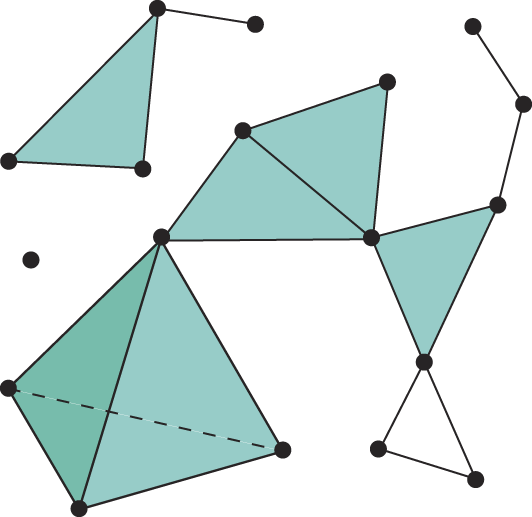
\includegraphics[width=0.25\textwidth]{simp_complex.png}
        \caption{Three dimensional simplicial complex.}
    \end{figure}

  \subsection{Persistent Homology}

\section{Applications of Topological Data Analysis}
  \subsection{Neuroscience}

  \subsection{Machine Learning}

    \begin{figure}
        \centering
        \includesvg[width=0.25\textwidth]{ff-net}
        \caption{Simple feed forward network. Attribution: 
                \href{https://commons.wikimedia.org/wiki/User:MartinThoma}{Martin Thoma}, 
                \href{https://creativecommons.org/licenses/by/3.0}{CC BY 3.0}}
    \end{figure}

\section{CONCLUSION}


\newpage
\section{ACKNOWLEDGMENT}
I'd like to acknowledge that I hate writing about things that I care absolutely nothing
about. Thank you.

\bibliographystyle{ieeetr}
\bibliography{refs}

\begin{wrapfigure}{l}{0.16\textwidth}
  \centering
  \vspace{-5mm}
  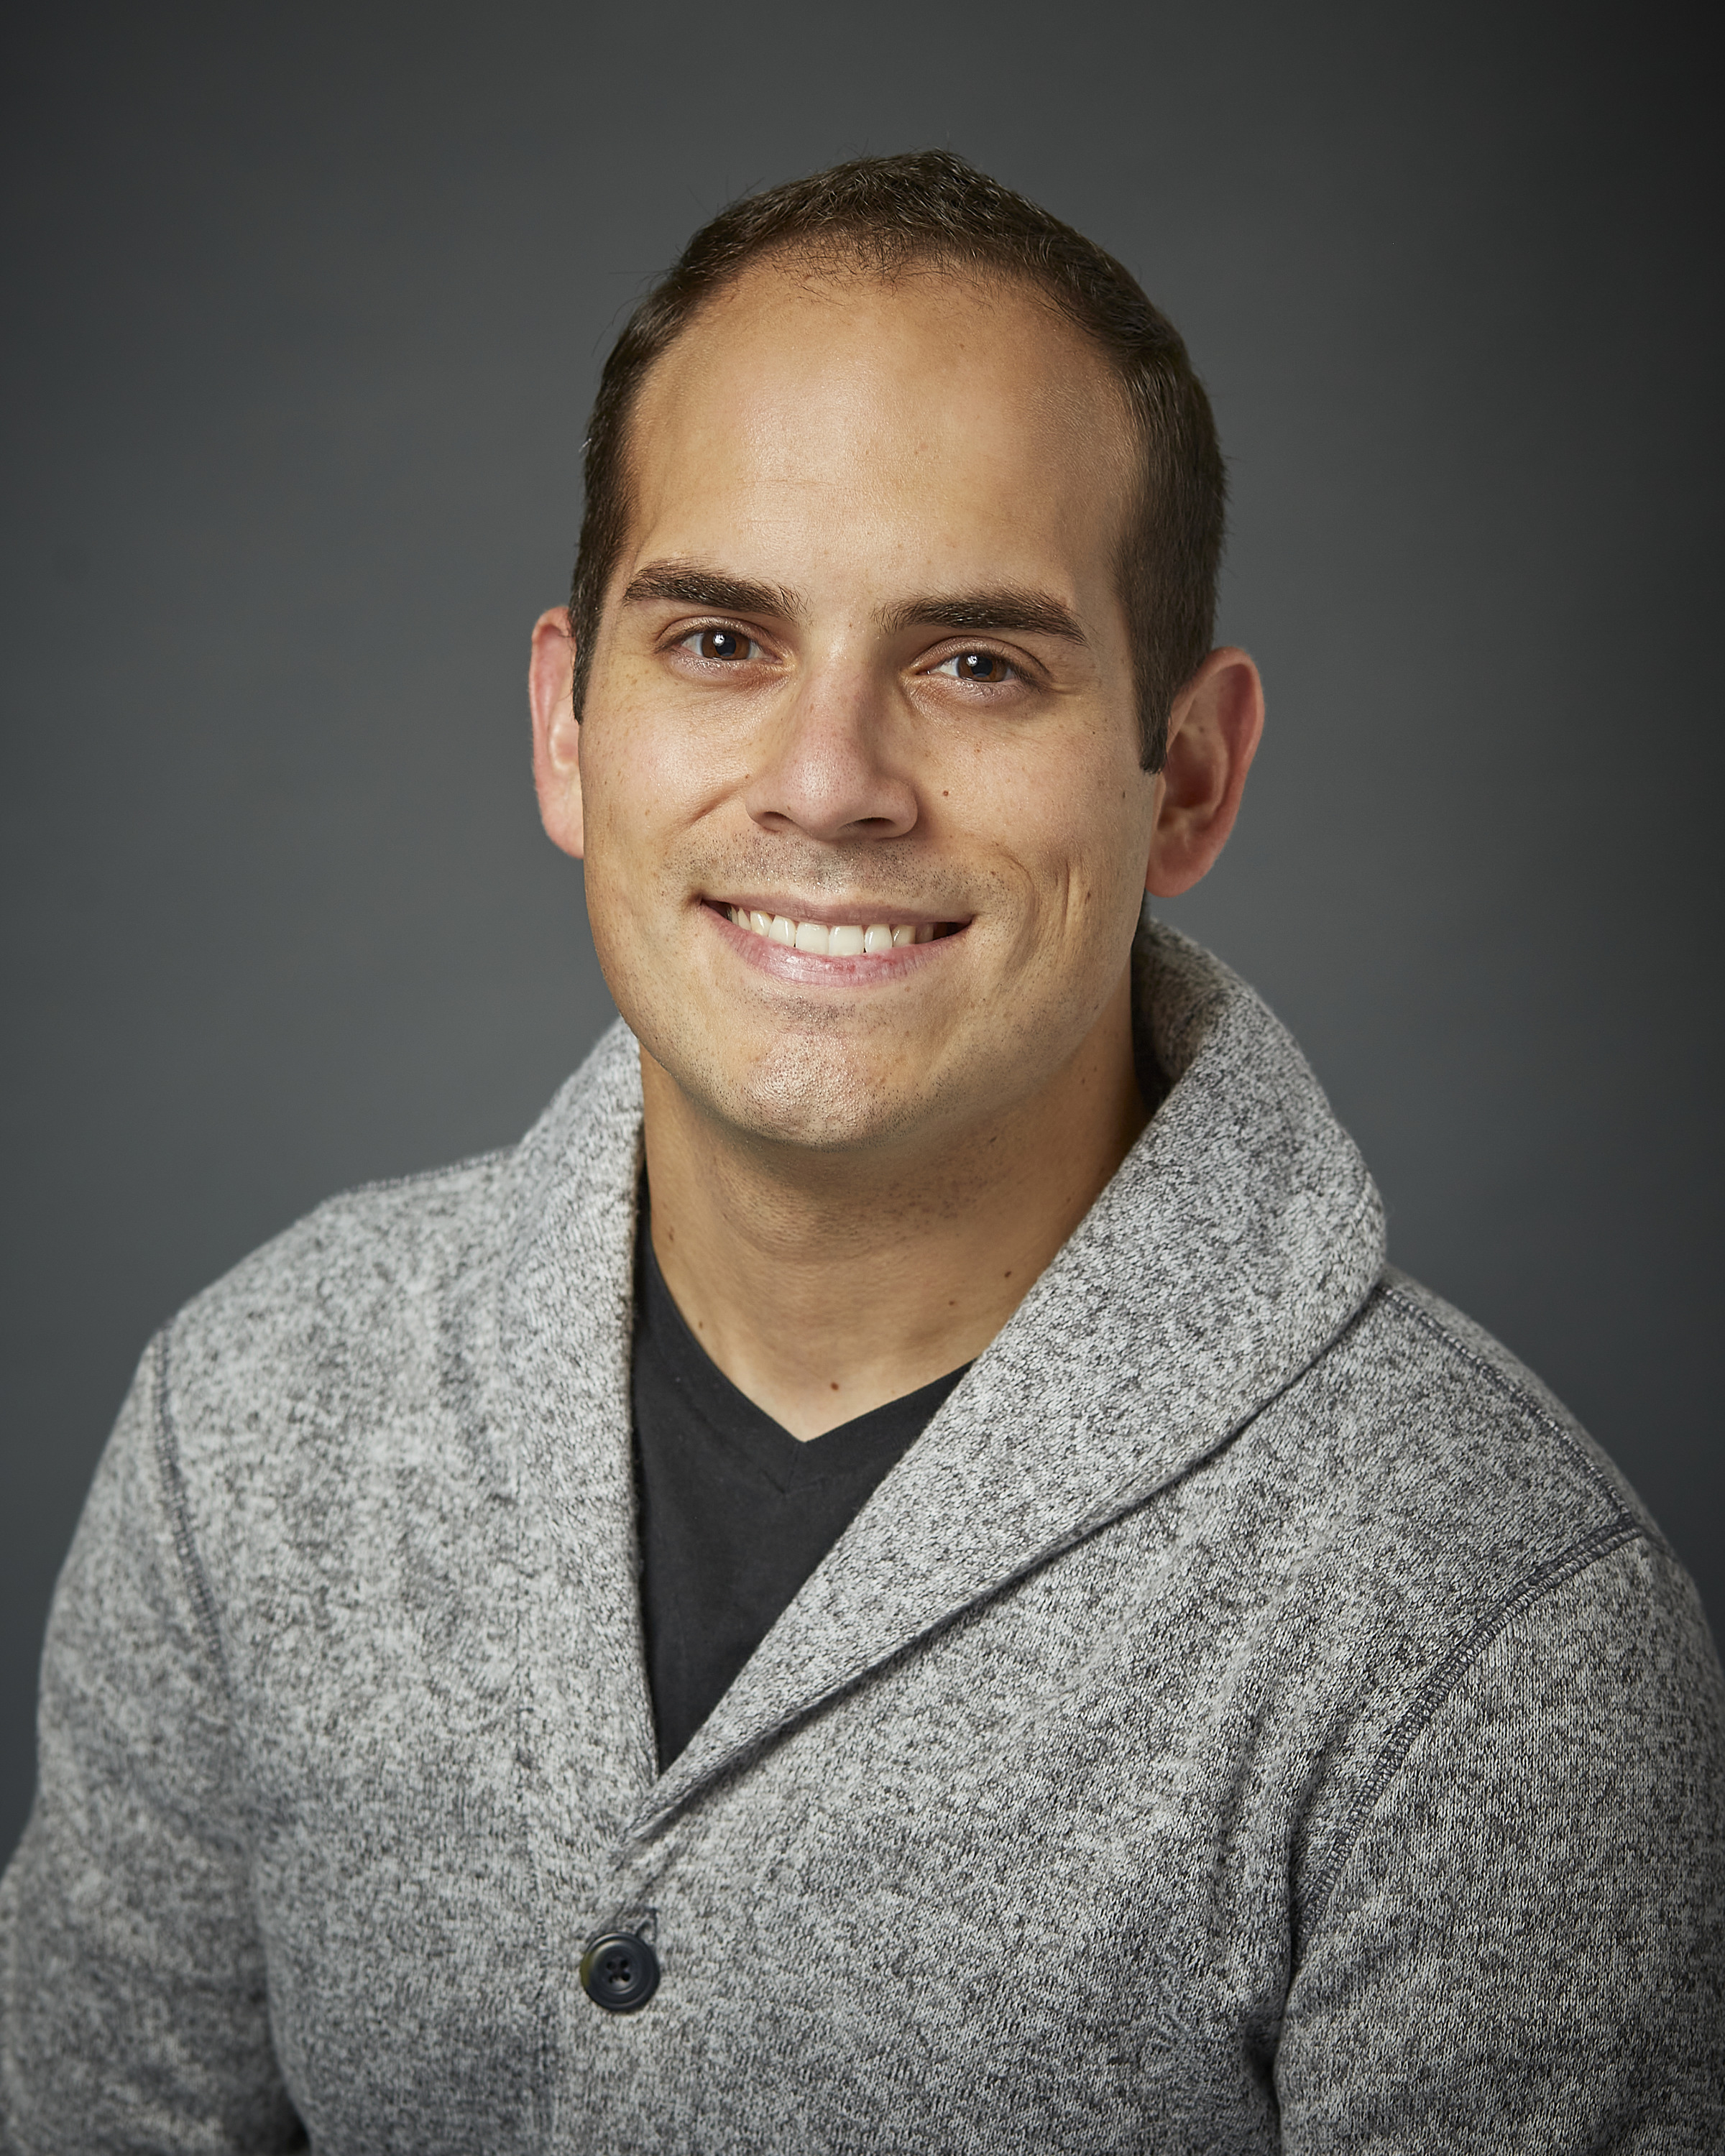
\includegraphics[width=0.18\textwidth]{portrait.jpg}
\end{wrapfigure}

\begin{IEEEbiography}{Tyler Trogden} 
  is a PhD candidate in Computer Science at BYU performing research in the
  field of machine learning and AI. When not working on his research, he enjoys
  spending time with his wife and family.
\end{IEEEbiography}

\end{document}